\documentclass[9pt]{beamer}
\setbeamertemplate{caption}[numbered]
\usetheme{Madrid}
%\usecolortheme{albatross} crane seagull seahorse
\usecolortheme{crane}
\usefonttheme[onlylarge]{structurebold}
\setbeamerfont*{frametitle}{size=\normalsize,series=\bfseries}
\setbeamertemplate{navigation symbols}{}
\usepackage{array}
\usepackage{textpos}
\usepackage{amsfonts}
\usepackage{amsmath}
\usepackage[export]{adjustbox}

\title{\huge Low Activity $^{241}$Am$^9$Be Source Run}
\author{Hao Qian}
%\author[Hao Qian]{Hao Qian\\{\small W.Masa, Peter Meyers}}
\institute{\it Princeton University}
\date{\today}
\begin{document}

\begin{frame}
\titlepage
\end{frame}

\begin{frame}{Motivation}
\begin{itemize}
\setbeamertemplate{itemize items}[bullet]
\item observe the $\alpha$ only channel from neutron capturing on TMB
\item study the neutron thermalization signal
\item Trigger Configuration study
\item help understand the neutron capturing as adding more TMB in the future
\end{itemize}
\end{frame}

%\begin{frame}{Geometry}
%\begin{itemize}
%\setbeamertemplate{itemize items}[bullet]
%\item 5$\%$ TMB in the scintillator 
%\item Source Holder (close to outer cryostat)
%	\begin{itemize}
%	\setbeamertemplate{itemize items}[default]
%	\item center position (-33.85, 3.35, -3.65) cm
%	\item inner length: 6.3 cm, inner diameter 2.7 cm
%	\item surround by a 2mm stainless steel outer layer
%	\item 2mm Lead inside layer 
%	\end{itemize}
%\item $^{241}$Am$^9$Be source at (-33.85, 0.4, -3.65)cm (disk shape)
%\item apply the cluster algorithm 	
%\item distinguish nuclear recoils from electron recoils by quenching factor (0.43)
%\item normalize the plots by the number of events
%\end{itemize}
%\end{frame}

%\begin{frame}{Quenching Factor}
%\begin{figure}
%\includegraphics[height = 7cm, width=\textwidth]{quenchingfactor_Ba133.png}
%\caption{The quenching factor larger than 0.43 is used to select electron recoils.}
%\end{figure}
%\end{frame}

\begin{frame}{Event Selection}
\begin{itemize}
\setbeamertemplate{itemize items}[bullet]
\item Runlist: 10974, 10975, 10976, 10977, 10978, 10983, 10985, 10987,
  10988, 10989, 10991, 10992, 10993, 10994, 10995, 10996, 10998, 10999,
  11000, 11002, 11003, 11005
%\item gps$\_$time$\_$diff = od$\_$timestamp - tpc$\_$timestamp + od$\_$cluster$\_$dtprompt  
%\item Cuts
\begin{exampleblock}{Cuts}
	\begin{itemize}
	\setbeamertemplate{itemize items}[default]
	\item pass multiplicity cut: od$\_$cluster$\_$pass$\_$multcut == 1  
	\item gamma events in TPC: tpc$\_$event$\_$type == 0
	\item neutron events in TPC: tpc$\_$event$\_$type == 1
	\item remove after pulses: od$\_$cluster$\_$dtprompt[0] $>$ 20ns
        \item skip LSV prompt:  od$\_$cluster$\_$dtprompt $>$ 1us
        \item events of interest:  od$\_$cluster$\_$dtprompt $<$ 50us
        \item select accidental events: 90us $<$ od$\_$cluster$\_$dtprompt $<$ 140us
	\end{itemize}
\end{exampleblock}	
\item Any other suggestions?
\end{itemize}
\end{frame}

\begin{frame}{$\alpha$ Generator}
\begin{itemize}
\setbeamertemplate{itemize items}[bullet]
\item $^{241}$Am$^9$Be source decay channels
\begin{align}
^{241}\rm{Am} \longrightarrow &  ^{237}\rm{Np}+ ^{4}\rm{He} + \gamma  \\
^{9}\rm{Be} + ^{4}\rm{He}  \longrightarrow & ^{12}\rm{C} + n (\sim 50\%)   \\
^{9}\rm{Be} + ^{4}\rm{He}  \longrightarrow  & ^{12}\rm{C}^* + n (\sim 50\%)  \\
	& ^{12}\rm{C}^* \longrightarrow ^{12}\rm{C} + \gamma(4.4\,MeV)
\end{align}
	\begin{itemize}
	\setbeamertemplate{itemize items}[default]
	\item 36$\%$ chance to produce neutron   
	\item 61$\%$ chance to produce neutron and 4.4 MeV $\gamma$
	\item 3$\%$ chance to produce neutron, 3.2 MeV and 4.4 MeV $\gamma$
	\end{itemize}
\item $^{10}$B captures neutrons via two channels:
\begin{align}
^{10}\rm{B} + n \longrightarrow  & ^{7}\rm{Li}(1015\, keV) + \alpha(1775\,keV)  & (6.4\%) \\
^{10}\rm{B} + n \longrightarrow  & ^{7}\rm{Li}^{*}(839\, keV) + \alpha(1471\, keV) &  \\
         & ^{7}\rm{Li}^{*}  \longrightarrow ^{7}\rm{Li} + \gamma(478\, keV)  & (93.7\%)
\end{align}
\end{itemize}
\end{frame}

\begin{frame}{Energy Spectrum from $^{241}$Am$^9$Be source decay channels from MC}
\begin{figure}
\includegraphics[height= 3 cm, width=.5\textwidth]{dau_gamma_only.pdf}
\includegraphics[height= 3 cm, width=.5\textwidth]{dau_neutron_only.pdf} \\
\includegraphics[height= 3 cm, width=.5\textwidth, left]{dau_all.pdf}
\caption{Top Left: Gamma Only channel. Top Right: Neutron Only channel. Bottom Left: Energy spectrum from all Channels  of $^{241}$Am$^9$Be source. Find more MC results \href{http://darkside-docdb.fnal.gov:8080/cgi-bin/RetrieveFile?docid=1074&filename=Alpha_Jan17.pdf&version=3}{\textcolor{green}{DocDB 1074}} }
\end{figure}
\end{frame}

\begin{frame}{TPC Gamma Energy Spectrum}
\begin{itemize}
\setbeamertemplate{itemize items}[bullet]
\item select the gamma event inside the TPC 
\item high energy gamma scatters and deposits energy in TPC
\item Based on both real data and MC, we still cannot get the full energy spectrum in TPC 
\end{itemize}
\begin{figure}
\includegraphics[height= 4cm, width=.5\textwidth]{tpc_gamma_total_s1_Jan24AM.png}
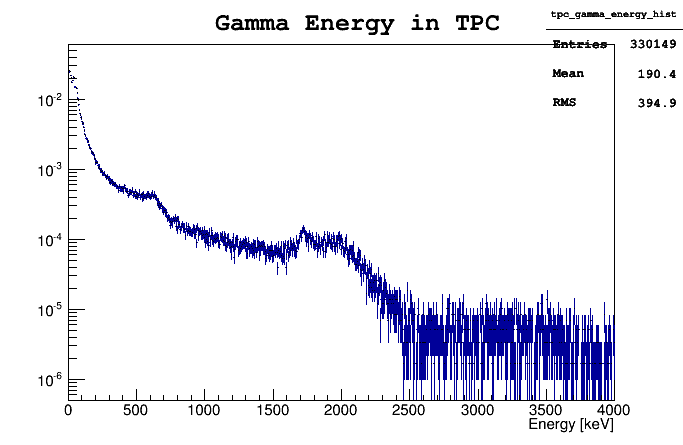
\includegraphics[height= 4cm, width=.5\textwidth]{tpc_gamma_energy_hist_Jan24AM.png}
\caption{Left: Gamma total s1 spectrum in TPC from real data. Right: MC Gamma Energy spectrum from all Channels  of $^{241}$Am$^9$Be source.}
\end{figure}
\end{frame}

\begin{frame}{Multiplicity Cut Study}
\begin{figure}
\includegraphics[height= 5cm, width=.8\textwidth]{multicut_Jan24AM.pdf}
\end{figure}
\begin{itemize}
\setbeamertemplate{itemize items}[bullet]
\item The peak at $\sim$250 PE comes from $\alpha$(1471keV)+$\gamma$(478keV) channel
\item $\alpha$(1775keV) only channel might appear at $\sim$20 PE 
\item 60keV $\gamma$ may leak from 2mm lead shield and deposits energy in LSV via compton scattering
\item need to subtract the 60keV $\gamma$ by accidental events 
\end{itemize}
\end{frame}

\begin{frame}{60KeV $\gamma$ from $^{241}$Am leaking out of the lead}
\begin{figure}
\includegraphics[height= 4cm, width=.5\textwidth]{nv_Am241_60keV_small_qene_Jan24AM.png}
\includegraphics[height= 4cm, width=.5\textwidth]{nv_Am241_60keV_small_time_Jan24AM.png}
\end{figure}
\begin{itemize}
\setbeamertemplate{itemize items}[bullet]
\item generate $^{241}$Am decay chain in the source holder
\item study the energy and time distribution in LSV
\end{itemize}
\end{frame}

\begin{frame}{Trigger on high energy TPC $\gamma$, neutron in veto}
\begin{itemize}
\setbeamertemplate{itemize items}[bullet]
\item event signature
	\begin{itemize}
	\setbeamertemplate{itemize items}[default]
	\item high energy $\gamma$ (from $^{12}$C de-excitation) goes into TPC
	\item select $\gamma$ only and avoid neutron going into TPC
	\item neutron capture in veto (prompt/delayed coincidence) 
	\item trigger on TPC, long veto gate ($\sim$50us)
	\end{itemize}
%\item understand from MC
%	\begin{itemize}
%	\setbeamertemplate{itemize items}[default]
%	\item residual $\gamma$ signal contamination in prompt (after selection)
%	\item full $^{241}$Am$^9$Be generator without $\gamma$ \\
%	  $\Rightarrow$ signal in veto from first cluster (what fraction is from $\gamma$, what is from neutron)
%	\end{itemize}
\item understand from 10n/s $^{241}$Am$^9$Be source campaign data
	\begin{itemize}
	\setbeamertemplate{itemize items}[default]
	\item residual $\gamma$ signal contamination in prompt (after selection)
	\item wait for high energy LSV prompt signals, then see neutron capture 
%	\item full $^{241}$Am$^9$Be generator without $\gamma$ \\
%	  $\Rightarrow$ signal in veto from first cluster (what fraction is from $\gamma$, what is from neutron)
	\end{itemize}
\item rate estimation for $\gamma$ in TPC, neutron entirely in veto
\end{itemize}
%\begin{table}[c]
%\centering
%\begin{tabular}{l | l | l | l }
%\hline \hline
% & $\gamma$ only channel & neutron only channel & all channels \\ \hline
%total events & 597315 & 856015 & 585906 \\ \hline
%Inside TPC events & 61428(10.3$\%$)  & 164858(19.3$\%$) & 142096(24.3$\%$) \\  \hline
%nuclear events &  0 & 91275(10.7$\%$) & 62650(10.7$\%$) \\ \hline
%pure nuclear events & 0 & 51557(6.0$\%$) & 33138(5.7$\%$) \\ \hline
%electron events & 61428(10.3$\%$) & 113301(13.2$\%$) & 108958(18.6$\%$) \\ \hline
%pure electron events & 61428(10.3$\%$) & 73583(8.6$\%$)  & 79446(13.6$\%$) \\ \hline
%residual gamma events & 25406(4.3$\%$) & 18563(2.2$\%$) & 25942(4.4$\%$) \\ \hline
%remain neutron events & 0 & 44875(5.2$\%$) & 28737(4.9$\%$) \\
%\hline \hline
%\end{tabular}
%\end{table}
\end{frame}	

\begin{frame}{Energy of Veto Clusters}
\begin{figure}
%\includegraphics[height= 4cm, width=\textwidth]{nv_neutron_alpha_small_ene_subtracted_Jan24AM.png}
\includegraphics[height= 4cm, width=\textwidth]{nv_gamma_alpha_small_ene_subtracted_Jan24AM.png}
\end{figure}
\begin{itemize}
\setbeamertemplate{itemize items}[bullet]
\item neutron get captures by $^{10}$B
\item \textcolor{blue}{blue} Lines in left plot is the accidental background 
\item the plots on the right has subtracted the accidental background 
\item the peak around 20PE comes from $\alpha$(1775keV) only channel (\textcolor{red}{peak 1})
\item the peak around 250PE comes from $\alpha$(1471keV)+$\gamma$(478keV) channel (\textcolor{green}{peak 2})
\item the branch ratio of \textcolor{red}{peak 1} to total increases to \textcolor{red}{9.3$\%$}, which is 6.4$\%$ Initially 
\end{itemize}
\end{frame}

\begin{frame}{MC Results of Energy Spectrum of last cluster from all channels}
\begin{figure}
\includegraphics[height= 4cm, width=.5\textwidth]{last_cluster_all_channels.pdf}
\includegraphics[height= 4cm, width=.5\textwidth]{smearing_v2_qenergy.pdf}
\end{figure}
\begin{itemize}
\setbeamertemplate{itemize items}[bullet]
\item neutron gets captures by $^{10}$B
\item the peak around 50keVee comes from $\alpha$(1775keV) only channel (\textcolor{red}{peak 1})
\item the peak around 420keVee comes from $\alpha$(1471keV)+$\gamma$(478keV) channel (\textcolor{green}{peak 2})
\item the branch ratio of \textcolor{red}{peak 1} to total increases to \textcolor{red}{15$\%$}, which is 6.4$\%$ Initially 
\item not sufficient data
\item any explaination?
\end{itemize}
\end{frame}

%\begin{frame}{MC Results Energy Spectrum of last cluster from all channels, Source holder rotates 90 degrees away}
%\begin{figure}
%\includegraphics[height= 4cm, width=.5\textwidth]{nv_alpha_qenergy_away.png}
%\includegraphics[height= 4cm, width=.5\textwidth]{nv_alpha_qenergy_smearing_away.png}
%\end{figure}
%\begin{itemize}
%\setbeamertemplate{itemize items}[bullet]
%\item source holder rotates 90 degrees away, new center position at (-101,-17,-3.65)cm
%\item the peak around 50keVee comes from $\alpha$(1775keV) only channel (\textcolor{red}{peak 1})
%\item the peak around 420keVee comes from $\alpha$(1471keV)+$\gamma$(478keV) channel (\textcolor{green}{peak 2})
%\item the branch ratio of \textcolor{red}{peak 1} to total becomes 7$\%$
%\item any explaination?
%\end{itemize}
%\end{frame}

%\begin{frame}{XY and Rho-Z distributions of neutron capture}
%\qquad   \qquad  \qquad next to cryostat  \qquad    \qquad \qquad   \qquad  \qquad rotate away by 90 degrees
%\begin{figure}
%\vspace{-1em}
%\includegraphics[height= 4cm, width=.5\textwidth]{nv_alpha_captrue_XY_hist.png}
%\includegraphics[height= 4cm, width=.5\textwidth]{nv_alpha_captrue_XY_away_hist.png} \\
%\includegraphics[height= 4cm, width=.5\textwidth]{nv_alpha_captrue_Zr_hist.png}  
%\includegraphics[height= 4cm, width=.5\textwidth]{nv_alpha_captrue_Zr_away_hist.png}
%\end{figure}
%\end{frame}

\begin{frame}{Neutron Capture Time}
\begin{itemize}
\setbeamertemplate{itemize items}[bullet]
\item gamma events in TPC: tpc$\_$event$\_$type == 0
%\item neutron events in TPC: tpc$\_$event$\_$type == 1
\item remove after pulses: od$\_$cluster$\_$dtprompt[0] $>$ 20ns
\item time window: 1us $<$ od$\_$cluster$\_$dtprompt $<$ 50us
\item the capture time is 21.1 us, which matches with calculation
\end{itemize}
\begin{figure}
%\includegraphics[height= 5cm, width=.8\textwidth]{nv_gamma_alpha_time_Jan24AM.png}
\includegraphics[height= 6cm, width=.8\textwidth]{nv_gamma_alpha_capture_time_Jan24AM.png}
\end{figure}
\end{frame}

%\begin{frame}{$\gamma$ energy spectrum in TPC}
%\begin{figure}
%\includegraphics[height= 7cm, width=\textwidth]{tpc_gamma_energy_list.pdf}
%\caption{The gamma energy spectrum of $^{241}$Am$^9$Be source.}
%\end{figure}
%\end{frame}

%\begin{frame}{residual $\gamma$ signal}
%\begin{itemize}
%\setbeamertemplate{itemize items}[default]
%\item time window [0,7us]
%\item gamma energy threshold 600keV
%\end{itemize}  
%\begin{figure}
%\includegraphics[height= 6cm, width=\textwidth]{nv_residual_qenergy_list.pdf}
%\caption{The gamma energy spectrum of $^{241}$Am$^9$Be source.}
%\end{figure}
%\end{frame}

%\begin{frame}{first cluster signal in veto}
%\begin{itemize}
%\setbeamertemplate{itemize items}[default]
%\item time window [0,500ns]
%\item energy threshold 600keV
%\end{itemize}  
%\begin{figure}
%\includegraphics[height= 6cm, width=\textwidth]{nv_first_qenergy_list.pdf}
%\caption{The gamma energy spectrum of $^{241}$Am$^9$Be source.}
%\end{figure}
%\end{frame}

%\begin{frame}{rate estimation in TPC}
%\begin{table}[c]
%\centering
%\begin{tabular}{l | l | l | l }
%\hline \hline
 %& $\gamma$ only channel & neutron only channel & all channels \\ \hline
%total events & 597315 & 856015 & 585906 \\ \hline
%Inside TPC events & 61428  & 164858 & 142096 \\  \hline
%nuclear events &  0 & 91275 & 62650 \\ \hline
%pure nuclear events & 0 & 51557 & 33138 \\ \hline
%electron events & 61428 & 113301 & 108958 \\ \hline
%pure electron events & 61428 & 73583  & 79446 \\ 
%\hline \hline
%\end{tabular}
%\caption{}
%\end{table}
%\end{frame}

%\begin{frame}{Veto Self-Trigger on neutron thermalization (neutron only channel)}
%\begin{itemize}
%\setbeamertemplate{itemize items}[bullet]
%\item goal: select neutron only channel where thermalization is entirely in veto
%\item event signature:
%	\begin{itemize}
%	\setbeamertemplate{itemize items}[default]
%	\item self-trigger on veto on neutron thermalization signal 
%	\item prompt/delayed coincidence in veto 
%	\item no signal in TPC at all
%	\end{itemize}
%\item understand from MC
%	\begin{itemize}
%	\setbeamertemplate{itemize items}[default]
%	\item after the ``no  signal in TPC" requirement how clean is the data set
%	 in terms of contamination from the 
%	n+$\gamma$ channel?
%	\item could one eliminate the n+$\gamma$ channel contamination by an energy cut on the prompt in veto? \\
%	hypothesis: \\
%		$\Rightarrow$ neutron thermalization only: small prompt signal  \\
%		$\Rightarrow$ n+$\gamma$: high prompt signal		
%	\end{itemize}
%\end{itemize}
%\end{frame}

%\begin{frame}{thermal $\gamma$ signal}
%\begin{itemize}
%\setbeamertemplate{itemize items}[default]
%\item time window [0,200ns]
%\item no cluster inside TPC
%\end{itemize}	
%\begin{figure}
%\includegraphics[height= 6cm, width=\textwidth]{nv_thermal_qenergy_list.pdf}
%\caption{The gamma energy spectrum of $^{241}$Am$^9$Be source.}
%\end{figure}
%\end{frame}

\begin{frame}{thermalization partially in TPC and veto}
\begin{itemize}
\setbeamertemplate{itemize items}[bullet]
\item goal: thermalization is partially in TPC and veto
\item event signature:
	\begin{itemize}
	\setbeamertemplate{itemize items}[default]
	\item self-trigger on veto on neutron thermalization signal or trigger on TPC
	\item neutron capture: delayed in veto
	\item select TPC F90 $>$ 0.6 or 0.7
	\item energy cut in veto(accept events below a certain threshold in veto based on trigger efficiency plot)	
	\end{itemize}
\begin{figure}
\includegraphics[height= 4 cm, width=.7\textwidth]{htrig15_eff.pdf}
\end{figure}
%\item understand from MC
\item understand the real data
	\begin{itemize}
	\setbeamertemplate{itemize items}[default]
	\item the remain thermalization signal (amplitude) in veto after neutron leaves TPC
	\item is that separated in time from the high energy gamma?
	\item what is the rate of this channel?
	\end{itemize}
\end{itemize} 
\end{frame}

\begin{frame}{TPC Neutron Energy Spectrum}
\begin{itemize}
\setbeamertemplate{itemize items}[bullet]
\item select the neutron event inside the TPC 
%\item high energy gamma scatters and deposits energy in TPC
%\item Based on both real data and MC, we still cannot get the full energy spectrum in TPC 
\end{itemize}
\begin{figure}
\includegraphics[height= 4cm, width=.5\textwidth]{tpc_neutron_total_s1_Jan24AM.png}
\includegraphics[height= 4cm, width=.5\textwidth]{tpc_neutron_qene_Jan24AM.png}
%\caption{Neutron total s1 spectrum in TPC from real data.}
\caption{Left: Neutron total s1 spectrum in TPC from real data. Right: MC Neutron Energy spectrum from all Channels  of $^{241}$Am$^9$Be source.}
\end{figure}
\end{frame}

\begin{frame}{Energy of Veto Clusters}
\begin{figure}
\includegraphics[height= 4cm, width=\textwidth]{nv_neutron_alpha_small_ene_subtracted_Jan24AM.png}
%\includegraphics[height= 4cm, width=\textwidth]{nv_gamma_alpha_small_ene_subtracted_Jan24AM.png}
\end{figure}
\begin{itemize}
\setbeamertemplate{itemize items}[bullet]
\item neutron get captures by $^{10}$B
\item Brown Lines in left plot is the accidental background 
\item the plots on the right has subtracted the accidental background 
\item the peak around 20PE comes from $\alpha$(1775keV) only channel (\textcolor{red}{peak 1})
\item the peak around 250PE comes from $\alpha$(1471keV)+$\gamma$(478keV) channel (\textcolor{green}{peak 2})
\item the branch ratio of \textcolor{red}{peak 1} to total increases to \textcolor{red}{21.6$\%$}, which is 6.4$\%$ Initially 
\end{itemize}
\end{frame}

%\begin{frame}{remain thermalization signal}
%\begin{itemize}
%\setbeamertemplate{itemize items}[default]
%\item select only nuclear cluster in TPC
%\item time window [-0.5 us,0.5 us]
%\item energy threshold 90.9keV, (light yield 0.55 p.e/keV)
%\end{itemize}	
%\begin{figure}
%\includegraphics[height= 6 cm, width=\textwidth]{nv_remain_qenergy_list.pdf}
%\end{figure}
%\end{frame}

\begin{frame}{Summary}
\begin{enumerate}
\item the configurations are suitable to select neutron captures on TMB and the 'alpha only'-channel
\item different configurations allow for slightly different selection focuses
\item need more data to get clear alpha peak 
%\item relative comparison between different configurations:
%	\begin{itemize}
%	\setbeamertemplate{itemize items}[default]
%	\item config 1: trigger on TPC & next to cryostat: closest to our physics case (n depositing energy in TPC $\rightarrow$capturing in veto)
%	\item config 3: self-trigger on HE gamma & rotated away: best light collection expected $\rightarrow$ optimized to see alpha peak
%	\item config. 2: only one change away from config. 1 and 3
%	\end{itemize}
\end{enumerate}
\end{frame}

%=================================BackUp Plots=============================


\begin{frame}{BackUp}
BackUp
\end{frame}

\begin{frame}{F90 vs S1 in TPC}
\begin{figure}
\includegraphics[height= 7 cm, width=\textwidth]{f90_tpc_total_s1_Jan24AM.png}
%\caption{The gamma energy spectrum of $^{241}$Am$^9$Be source.}
\end{figure}
\end{frame}

\begin{frame}{Coincidence $\gamma$ Trigger signal in veto}
-200ns $<$ od$\_$cluster$\_$dtprompt $<$ 50us, od$\_$cluster$\_$pass$\_$multcut =1,  tpc$\_$event$\_$type =0

\begin{figure}
\includegraphics[height= 7 cm, width=\textwidth]{nv_gamma_coincidence_Jan24AM.png}
%\caption{The gamma energy spectrum of $^{241}$Am$^9$Be source.}
\end{figure}
\end{frame}

\begin{frame}{Delay $\gamma$ Trigger signal in veto}
0 $<$ od$\_$cluster$\_$dtprompt $<$ 50us, od$\_$cluster$\_$pass$\_$multcut =1,  tpc$\_$event$\_$type =0

\begin{figure}
\includegraphics[height= 7 cm, width=\textwidth]{nv_gamma_delay_Jan24AM.png}
%\caption{The gamma energy spectrum of $^{241}$Am$^9$Be source.}
\end{figure}
\end{frame}

\begin{frame}{After $\gamma$ Trigger signal in veto}
200ns $<$ od$\_$cluster$\_$dtprompt $<$ 50us, od$\_$cluster$\_$pass$\_$multcut =1,  tpc$\_$event$\_$type =0

\begin{figure}
\includegraphics[height= 7 cm, width=\textwidth]{nv_gamma_after_Jan24AM.png}
%\caption{The gamma energy spectrum of $^{241}$Am$^9$Be source.}
\end{figure}
\end{frame}

\begin{frame}{First $\gamma$ Trigger signal in veto}
0 $<$ od$\_$cluster$\_$dtprompt $<$ 500ns, od$\_$cluster$\_$pass$\_$multcut =1,  tpc$\_$event$\_$type =0

\begin{figure}
\includegraphics[height= 7 cm, width=\textwidth]{nv_gamma_first_Jan24AM.png}
%\caption{The gamma energy spectrum of $^{241}$Am$^9$Be source.}
\end{figure}
\end{frame}

\begin{frame}{Prompt $\gamma$ Trigger signal in veto}
-200ns $<$ od$\_$cluster$\_$dtprompt $<$ 0, od$\_$cluster$\_$pass$\_$multcut =1,  tpc$\_$event$\_$type =0

\begin{figure}
\includegraphics[height= 7 cm, width=\textwidth]{nv_gamma_prompt_Jan24AM.png}
%\caption{The gamma energy spectrum of $^{241}$Am$^9$Be source.}
\end{figure}
\end{frame}

\begin{frame}{Alpha $\gamma$ Trigger signal in veto}
1us $<$ od$\_$cluster$\_$dtprompt $<$ 50us, od$\_$cluster$\_$pass$\_$multcut =1,  tpc$\_$event$\_$type =0,od$\_$cluster$\_$dtprompt[0] $>$ 20ns

\begin{figure}
\includegraphics[height= 7 cm, width=\textwidth]{nv_gamma_alpha_Jan24AM.png}
%\caption{The gamma energy spectrum of $^{241}$Am$^9$Be source.}
\end{figure}
\end{frame}

\begin{frame}{Late $\gamma$ Trigger signal in veto}
90us $<$ od$\_$cluster$\_$dtprompt $<$ 140us, od$\_$cluster$\_$pass$\_$multcut =1,  tpc$\_$event$\_$type =0

\begin{figure}
\includegraphics[height= 7 cm, width=\textwidth]{nv_gamma_late_Jan24AM.png}
%\caption{The gamma energy spectrum applied with single electron scattering selection.}
\end{figure}
\end{frame}

%********************Neutron Trigger***************************

\begin{frame}{Coincidence Neutron Trigger signal in veto}
-200ns $<$ od$\_$cluster$\_$dtprompt $<$ 50us, od$\_$cluster$\_$pass$\_$multcut =1,  tpc$\_$event$\_$type =1

\begin{figure}
\includegraphics[height= 7 cm, width=\textwidth]{nv_neutron_coincidence_Jan24AM.png}
%\caption{The neutron energy spectrum of $^{241}$Am$^9$Be source.}
\end{figure}
\end{frame}

\begin{frame}{Delay Neutron Trigger signal in veto}
0 $<$ od$\_$cluster$\_$dtprompt $<$ 50us, od$\_$cluster$\_$pass$\_$multcut =1,  tpc$\_$event$\_$type =1

\begin{figure}
\includegraphics[height= 7 cm, width=\textwidth]{nv_neutron_delay_Jan24AM.png}
%\caption{The neutron energy spectrum of $^{241}$Am$^9$Be source.}
\end{figure}
\end{frame}

\begin{frame}{After Neutron Trigger signal in veto}
200ns $<$ od$\_$cluster$\_$dtprompt $<$ 50us, od$\_$cluster$\_$pass$\_$multcut =1,  tpc$\_$event$\_$type =1

\begin{figure}
\includegraphics[height= 7 cm, width=\textwidth]{nv_neutron_after_Jan24AM.png}
%\caption{The neutron energy spectrum of $^{241}$Am$^9$Be source.}
\end{figure}
\end{frame}

\begin{frame}{First Neutron Trigger signal in veto}
0 $<$ od$\_$cluster$\_$dtprompt $<$ 500ns, od$\_$cluster$\_$pass$\_$multcut =1,  tpc$\_$event$\_$type =1

\begin{figure}
\includegraphics[height= 7 cm, width=\textwidth]{nv_neutron_first_Jan24AM.png}
%\caption{The neutron energy spectrum of $^{241}$Am$^9$Be source.}
\end{figure}
\end{frame}

\begin{frame}{Prompt Neutron Trigger signal in veto}
-200ns $<$ od$\_$cluster$\_$dtprompt $<$0, od$\_$cluster$\_$pass$\_$multcut =1,  tpc$\_$event$\_$type =1

\begin{figure}
\includegraphics[height= 7 cm, width=\textwidth]{nv_neutron_prompt_Jan24AM.png}
%\caption{The neutron energy spectrum of $^{241}$Am$^9$Be source.}
\end{figure}
\end{frame}

\begin{frame}{Alpha Neutron Trigger signal in veto}
1us $<$ od$\_$cluster$\_$dtprompt $<$ 50us, od$\_$cluster$\_$pass$\_$multcut =1,  tpc$\_$event$\_$type =1,od$\_$cluster$\_$dtprompt[0] $>$ 20ns

\begin{figure}
\includegraphics[height= 7 cm, width=\textwidth]{nv_neutron_alpha_Jan24AM.png}
%\caption{The neutron energy spectrum of $^{241}$Am$^9$Be source.}
\end{figure}
\end{frame}

\begin{frame}{Late Neutron Trigger signal in veto}
90us $<$ od$\_$cluster$\_$dtprompt $<$ 140us, od$\_$cluster$\_$pass$\_$multcut =1,  tpc$\_$event$\_$type =1

\begin{figure}
\includegraphics[height= 7 cm, width=\textwidth]{nv_neutron_late_Jan24AM.png}
%\caption{The neutron energy spectrum applied with single electron scattering selection.}
\end{figure}
\end{frame}



\end{document}
